\documentclass[paper=a4,fontsize=11pt]{temp} % KOMA-article 
\usepackage{array}

\begin{document}
\sepspace
\begin{minipage}{.15\linewidth}
  % 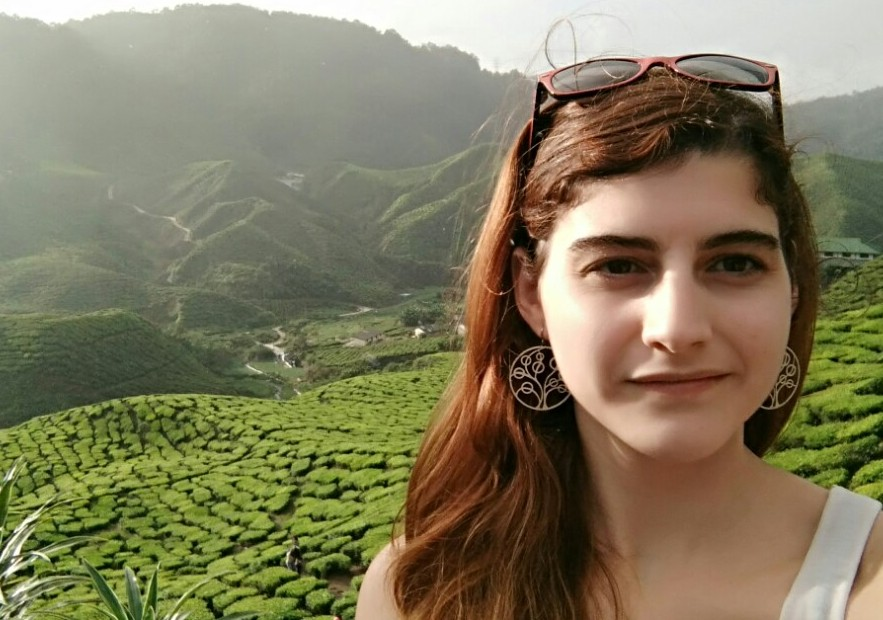
\includegraphics[width=1.4\textwidth]{ana2}
   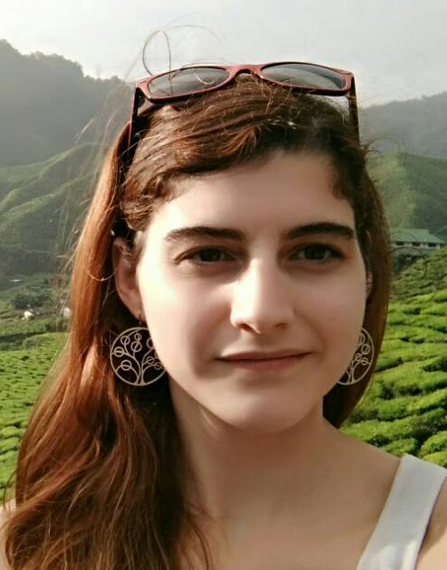
\includegraphics[width=\textwidth]{ana}
\end{minipage}      
\begin{minipage}{0.75\linewidth}
   \MyName{Ana Garcia del Molino}
   \sepspace
   \noindent
   
   \hfill    
   \begin{tabular}[width=\textwidth]{@{}cl@{}}
   \setlength{\tabcolsep}{12pt}
   \begin{tabular}{>{\centering\arraybackslash}p{.55\textwidth}} \centering \small \textit{I am in my $2$nd year of PhD. at I2R and NTU, Singapore, currently working on the summarization of egocentric videos. \\My research interests are in the areas of computer vision, pattern recognition and cognitive vision.} \end{tabular}
   & \setlength{\tabcolsep}{5pt} \begin{tabular}{@{}cl@{}}
    
\includegraphics[height=2ex]{IMG/icons/profile} & Spain, May 17th 1990  \\
    
\includegraphics[height=2ex]{IMG/icons/mail9} & a.g.delmolino@ieee.org  \\
    
\includegraphics[height=2ex]{IMG/icons/telephone1} &(+65) 86021449 \\    
    
\includegraphics[height=2ex]{IMG/icons/social6}  &  ana.garcia.del.molino\\    
    
\includegraphics[height=2ex]{IMG/icons/map5}  & Singapore   
   \end{tabular}
 \end{tabular}
   %\hfill yourwebsite.com
   
   %\hfill (+351)93123123123  
 
\end{minipage}


\NewPart{Work experience}{}
\noindent


\workEntry{Institute for Infocomm Research, A*STAR}{Aug 2014 - Today}{Research Assistant}{Ph.D. student position at the REVIVE project. Research topic: “Visual Memory and Summarization from First Person View”} {IMG/A-STAR}
\sepspace

\workEntrySmall{Nanyang Techonological University}{Fall 2016}{Teaching Assistant}{Teacher at the Algorithms CE2001 module lab.}{IMG/NTUE}

\sepspace

\workEntrySmall{PricewaterhouseCoopers}{Nov 2013 - Aug 2014}{SPA Auditor}{Systems \& Process Assurance Auditor for annual audits in several multinational companies.}{IMG/pwc}

\sepspace

\workEntry{National Institute of Informatics, Tokyo}{Mar 2013 - Sep 2013 }{Research Intern}{Intern at Shin’ichi Satoh’s
group. Participation in TRECVID Instance Search 2013 while researching for my Master Thesis.} {IMG/nii2}

\sepspace

\workEntrySmall{UPC Image and Video Processing Group}{Apr 2012 - Mar 2013}{Research Intern}{Research in several projects for Mediapro, including a basketball tracking system.}{IMG/upc}


\sepspace

\workEntrySmall{Centre Municipal de Vela Barcelona}{2008-2011}{Sailing Instructor}{Summer sailing courses for kids of all ages and adults.}{IMG/cmv}


\NewPart{Education}{}
\noindent


\EducationEntry{Phd. in Cognitive Systems and Visual Computing}{Jan 2015 - Today}{School of Computer Science and Engineering, NTU, Singapore}{My research focuses on the integration of cognitive models into computer vision systems, towards
efficient visual memory organization and retrieval.
GPA 4.63/5.} {IMG/NTUE}

\sepspace


\EducationEntry{MSc. Telecommunications Engineering}{Sep 2008 - Sep 2013}{TelecomBCN (ETSETB, UPC Barcelona Tech), Spain}{Bachelor and Master Degree with specialty in Communications.\\9.5/10 qualification for my Thesis, average grade of 7.33/10, order 33/144 and efficiency of 0.94.} {IMG/logo_telecom_S}


%\sepspace

\NewPart{Skills \& Interests}{}
\hspace{3mm}
\begin{minipage}[t]{0.33\textwidth} 

\begin{tabular}[t]{ l l }
\flag{IMG/flag/es}  & Native Speaker \\
\flag{IMG/flag/cat} & Native Speaker \\
\flag{IMG/flag/gb}  & TOEFL iBT 103/120 \\
%Professional Proficiency \\
\flag{IMG/flag/fr}  & European B2.2\\%Conversational level \\
%Professional user \\
\flag{IMG/flag/de}  & Basic European A1\\
\end{tabular}

\sepspace

\end{minipage}
%
\begin{minipage}[t]{0.66\textwidth} 

\begin{tabular}[t]{l l}
\softwareb{IMG/soft/computer}  	 &\small \begin{tabular}[t]{@{}l@{}} Matlab, Python, C++, image library OpenCV.\\
Linux user. Proficient in both Office tools and \LaTeX\\
Basic knowledge in video and audio editors. \end{tabular} \vspace{.7ex}
\\
\softwareb{IMG/hobbie}  &\small\setlength\extrarowheight{-1ex}\begin{tabular}[t]{@{}p{.8\linewidth}@{}}
sailing, traveling, volleyball, board games, cooking, painting, reading, playing the flute and the piano, cinema, opera... 
\end{tabular} \\
\end{tabular}
\end{minipage}

\setlength\extrarowheight{-1ex}
\vspace{1ex}
\begin{tabular}{l l}
%
\softwareb{IMG/people}  &\small  \begin{tabular}[t]{@{}p{.85\linewidth}@{}}
Member of the IEEE; Vice-President of the IEEE Barcelona Student Branch in 2011-2013;\\ organizer of the National Student Branch Congress 2012 in Barcelona, Spain.\vspace{1ex}\\
 Active member in the association DAT, the Student’s Delegation in my undergrad college;\\
 member of the student group at ETSETB’s Evaluation Committee and Board during my studies.\vspace{1ex}\\
 Intern at the International Student Office of my university the year 2012.\end{tabular} 
\end{tabular}

%
\pagebreak
\sepspace

\NewPart{Publications}{}
\hspace{3mm}
\begin{minipage}{0.04\linewidth}
        \hspace{\linewidth}
		\end{minipage}%  
   \begin{minipage}{0.88\linewidth}
   \noindent\hangindent=2em\hangafter=1 
    A. G. del Molino, X. Boix, and J. H. Lim, ``Active Video Summarization to Meet the User’s Preferences,'' in \textit{Thirty First AAAI Conference on Artificial Intelligence}. AAAI, 2017. In press.
    \sepspace
    
    \noindent\hangindent=2em\hangafter=1 
    A. G. del Molino, C. Tan, J. H. Lim and A. H. Tan, ``Summarization of Egocentric Videos: A Comprehensive Survey,'' in \textit{IEEE Transactions on Human-Machine Systems}. IEEE, 2016. In press.\sepspace
    
       \noindent\hangindent=2em\hangafter=1 
    A. G. del Molino, ``First Person View Video Summarization Subject to the User Needs,'' in \textit{Proceedings of the 2016 ACM on Multimedia Conference,} pp. 1440-1444. ACM, 2016.
\sepspace 

\noindent\hangindent=2em\hangafter=1 
    A. G. del Molino, Q. Xu, and J. H. Lim, ``Describing Lifelogs with Convolutional Neural Networks: A Comparative Study,'' in \textit{Proceedings of the first Workshop on Lifelogging Tools and Applications,} pp. 39-44. ACM, 2016.
	\sepspace
    
       \noindent\hangindent=2em\hangafter=1 
   A. G. del Molino, B. Mandal, L. Li, and J. H. Lim, ``Organizing and Retrieving Episodic Memories from First Person View," in \textit{International Conference on Multimedia \& Expo Workshops (ICMEW),} pp. 1-6. IEEE, 2015. %  	1st  International Workshop on Wearable and Ego-vision Systems for Augmented Experience, International Conference on Multimedia and Expo, Turin, Italy, 2015.

   \end{minipage}        
\sepspace

\NewPart{Honors \& Awards}{}
\hspace{3mm}
\begin{minipage}[t]{0.45\textwidth}
\AwardEntry{SINGA Scholarship}{Jan 2015}{Singaporean scholarship for the PhD. joint program between A*STAR and NTU.} {IMG/Logo_of_A-STAR}
\end{minipage}
\hspace{0.02\textwidth}
\begin{minipage}[t]{0.45\textwidth}
\AwardEntry{Obra Social "La Caixa"}{Apr 2015}{Scholarship to cover additional conference and travel expenses during my PhD.} {IMG/lacaixa}
\end{minipage}

\sepspace

\NewPart{Referees}{}
\hspace{3mm}
\begin{minipage}[t]{0.45\textwidth}
\RefereeEntry{LIM Joo-Hwee}{I2R, A*STAR}{My PhD. research supervisor \\joohwee@i2r.a-star.edu.sg} {pics/limjoohwee}
\end{minipage}
\hspace{0.02\textwidth}
\begin{minipage}[t]{0.45\textwidth}
\RefereeEntry{TAN Ah-Hwee}{SCSE, NTU}{My PhD. accademic supervisor\\ASAHTan@ntu.edu.sg} {pics/ahhwee}
\end{minipage}
 \sepspace
 
\begin{minipage}[t]{0.45\textwidth}
\RefereeEntry{Xavi Giro-i-Nieto}{ETSETB, UPC}{My MSc. supervisor and councelor\\xavier.giro@upc.edu } {pics/xavi}
\end{minipage}
\hspace{0.02\textwidth}
\begin{minipage}[t]{0.45\textwidth}
\RefereeEntry{Ferran Marques}{ETSETB, UPC}{My BSc. and MSc. mentor\\ferran.marques@upc.edu } {pics/ferran}
\end{minipage}
\sepspace

%%% References
%%% ------------------------------------------------------------

\end{document}
